%------------------------------------------------------------------------------
% Author(s):
% Varaun Ramgoolie
%
% Copyright:
%  Copyright (C) 2020 Brad Bachu, Arjun Mohammed, Varaun Ramgooie, Nicholas Sammy
%
%  This file is part of Applied-Mathematics-Unit2 and is distributed under the
%  terms of the MIT License. See the LICENSE file for details.
%
%  Description:
%     Year: 2016
%     Module: 3
%     Question: 5
%------------------------------------------------------------------------------

%------------------------------------------------------------------------------
% 5 a
%------------------------------------------------------------------------------

\begin{subquestions}

\subquestion
We are given a fixture which is attached to a horizontal ceiling by two strings.
\begin{subsubquestions}

\subsubquestion

\textbf{\textit{Sketch and Translate:}} \\ \\
\begin{figure}[H]
	\begin{center}
		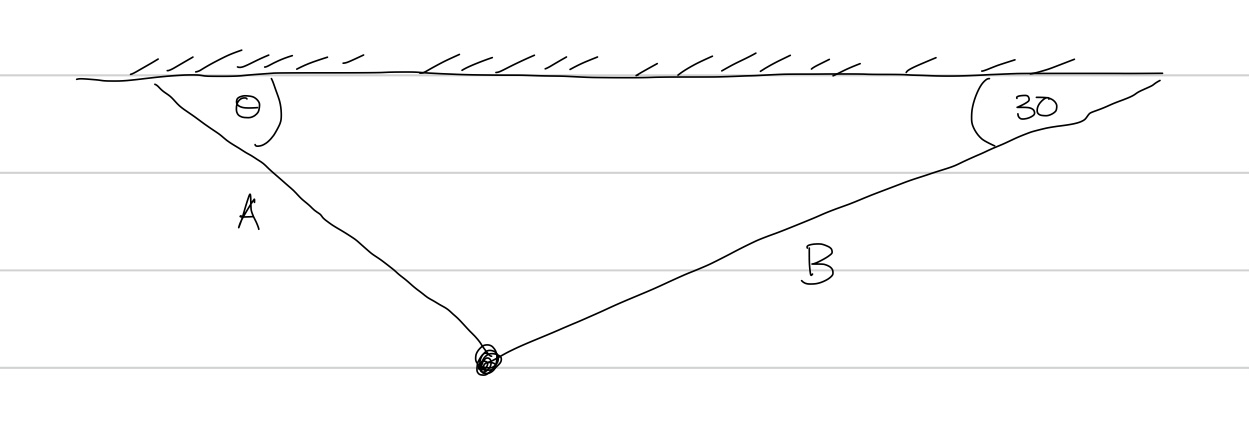
\includegraphics[scale=0.25]{../2016/figures/2016q5-1}
		\caption{\label{2016:q5:Sketch1} Fixture hanging from ceiling.}
	\end{center}
\end{figure}
If we assume that the fixture is in equilibrium, we should think about how we can represent the weight of the fixture in terms of the forces on the strings $A$ and $B$.




\textbf{\textit{Simplify and Diagram:}} \\ \\
\begin{figure}[H]
	\begin{center}
		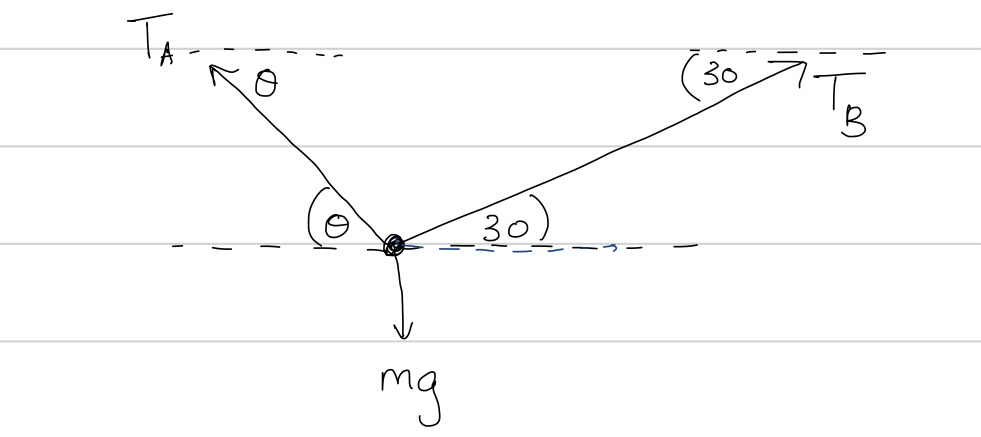
\includegraphics[scale=0.25]{../2016/figures/2016q5-2}
		\caption{\label{2016:q5:Diagram1} Free body diagram of the fixture.}
	\end{center}
\end{figure}
We will consider the fixture as a point particle. Let us represent the forces on the fixture as,
\begin{itemize}
	\item $T_A$ which is the tension on string A,
	\item $T_B$ which is the tension on string B, 
	\item $W$ which is the weight of the fixture.
\end{itemize}
We are given the magnitude of $T_A$. We should aim to resolve all of the forces on the fixture in terms of their $x$ and $y$ components and use Newton's Second Law to solve for $W$.




\textbf{\textit{Represent Mathematically:}} \\ \\
As the particle is in equilibrium, we know that the Resultant Force $F_R$ on the particle is 0. By Newton's Second Law, we get that,
\begin{align}
	F_R = \sum \vec{F} & = 0 \nn \\
	\implies \sum F \xhat & = 0 \xhat \label{2016:q5:XEqn1} \\
	& \text{and} \nn \\
	\implies \sum F \yhat & = 0 \yhat \label{2016:q5:YEqn1} \,.
\end{align}

We can represent our forces on the fixture as,
\begin{align}
	\vec{T_A} & = -|T_A|\cos(\theta)\xhat +|T_A|\sin(\theta)\yhat  \\
	\vec{T_B} & = |T_B|\cos(30)\xhat+|T_B|\sin(30)\yhat  \\ 
	\vec{W} & = -|W|\yhat \,.
\end{align}




\textbf{\textit{Solve and Evaluate:}} \\ \\
Using \req{2016:q5:XEqn1}, by substituting our values, we get that,
\begin{align}
	\sum F \xhat & = 0 \xhat \nn \\
	-|T_A|\cos(\theta)\xhat +  |T_B|\cos(30)\xhat & = 0 \xhat \nn \\
	-50\cos(\theta) + \frac{\sqrt{3}}{2}|T_B| & = 0 \nn \\
	\implies |T_B| & = \frac{100\cos(\theta)}{\sqrt{3}} \,.
\end{align}

Using \req{2016:q5:YEqn1}, we can find that,
\begin{align}
	\sum F \yhat & = 0 \yhat \nn \\
	|T_A|\sin(\theta)\yhat + |T_B|\sin(30)\yhat -|W|\yhat & = 0 \yhat \nn \\
	50\sin(\theta) + \left(\frac{100\cos(\theta)}{\sqrt{3}}\right)\sin(30) & = |W| \nn \\
	50\sin(\theta) + \left(\frac{100\cos(\theta)}{\sqrt{3}}\right)\left(\frac{1}{2}\right) & = |W|\nn \\
	50 \left(\sin(\theta) + \frac{\cos(\theta)}{\sqrt{3}}\right) & = |W| \,.
\end{align}

In our Second Solution, we will use Lami's Theorem to achieve the same result.

%------------------------------------------------------------------------------

\subsubquestion
From (a)(i), we have already shown that,
\begin{equation}
	|T_B| = \frac{100\cos(\theta)}{\sqrt{3}} \,.
\end{equation}

\end{subsubquestions}

%------------------------------------------------------------------------------
% 5 b
%------------------------------------------------------------------------------

\subquestion

\begin{subsubquestions}
	
\subsubquestion 

See \rfig{2016:q5:Diagram2}
\begin{figure}[H]
	\begin{center}
		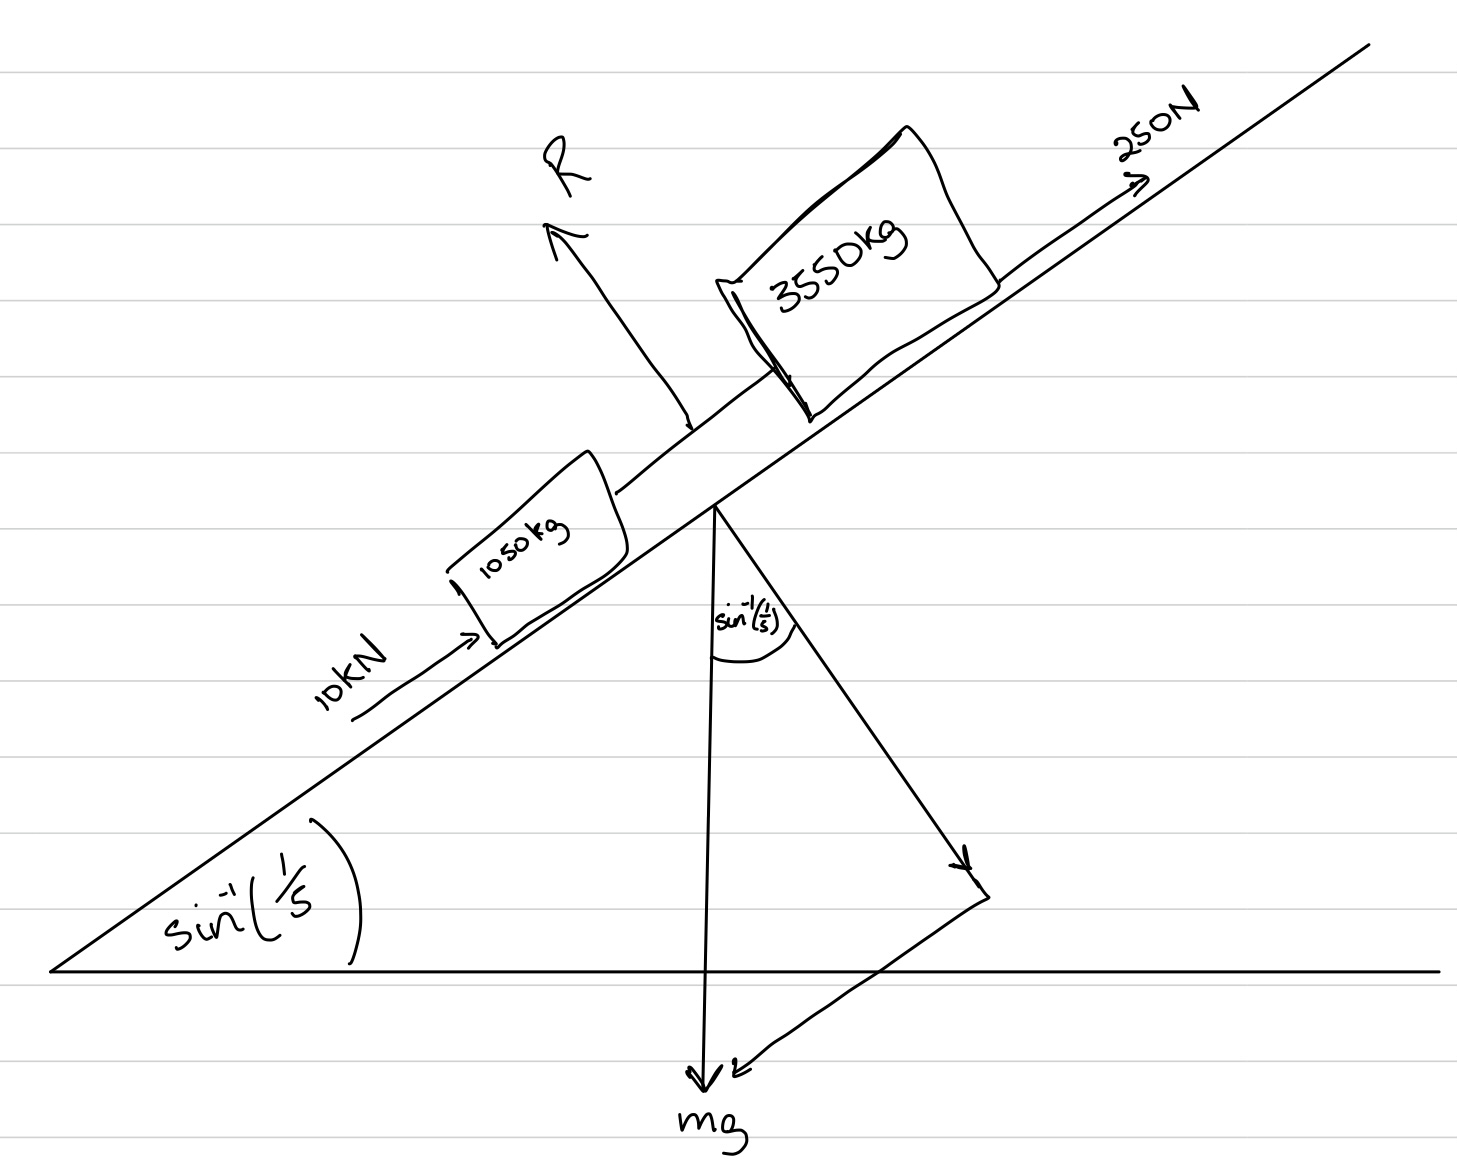
\includegraphics[scale=0.25]{../2016/figures/2016q5-3}
		\caption{\label{2016:q5:Diagram2} Wrecker after engine shuts off.}
	\end{center}
\end{figure}

%------------------------------------------------------------------------------

\subsubquestion

\textbf{\textit{Simplify and Diagram:}} \\ \\
We can consider \rfig{2016:q5:Diagram2} to understand what is happening with the wrecker. As the wrecker is moving down the plane, we know that the track resistance and the braking force must both act up the plane. Let us represent the forces on the wrecker as,
\begin{itemize}
	\item $W$, which is the weight on the wrecker and train of buses,
	\item $F_b$, which is the braking force, 
	\item $F_t$, which is the track resistance,
	\item $R$, which is the normal reaction force of the wrecker and train of buses.
\end{itemize}
We will assume that the wrecker and train of buses act as a point particle. In order to find the decelerating force, we will resolve the forces parallel to the plane and find the resultant force.




\textbf{\textit{Represent Mathematically:}} \\ \\
By resolving the forces in the $x$ and $y$ directions, we get that,
\begin{align}
	\vec{W} & = |W|\sin(\arcsin(0.2))\xhat - |W|\cos(\arcsin(0.2))\yhat \nn \\
	\vec{F_b} & = -10000\xhat \nn \\
	\vec{F_t} & = -250\xhat \nn \\
	\vec{R} & = |R|\yhat \,.
\end{align}

We also know that,
\begin{equation}
	|W|=mg \,.
\end{equation}




\textbf{\textit{Solve and Evaluate:}} \\ \\
The resultant force in the $x$ direction, $F_x$, can be given as,
\begin{align}
	F_x = \sum \vec{F}\xhat & = |W|\sin(\arcsin(0.2))\xhat -10000\xhat-250\xhat \nn \\
	F_x & = 0.2mg -10000-250 \nn \\
	    & = 0.2(4600)(10) -10000-250 \nn \\
	    & = -1050 N \,.
\end{align}

This value is negative as the force is causing the body to decelerate and thus, must be directed in the opposite way to the direction of motion.

%------------------------------------------------------------------------------

\subsubquestion
\textbf{\textit{Simplify and Diagram:}} \\ \\
We can consider \rfig{2016:q5:Diagram2} to understand what is happening. By using Newton's Second Law, we can find the deceleration of the particle. We can then use the equations of motion in order to find the time taken to reach the speed of 44kmh$^{-1}$.




\textbf{\textit{Represent Mathematically:}} \\ \\
From Newton's Second law, we get that,\footnote{We are considering the resultant force in the $x$ direction, $F_x$.}
\begin{align}
	F_x & = ma \nn \\
	\implies a & = \frac{F_x}{m} \,.
\end{align}

As we are given the initial and final velocities and we can find the acceleration, we will use,
\begin{align}
	v & = u + at \nn \\
	\implies t & = \frac{v-u}{a} \label{2016:q5:MotionEqn}\,.
\end{align}




\textbf{\textit{Solve and Evaluate:}} \\ \\
Firstly, we must convert the initial velocities into ms$^{-1}$ as,
\begin{align}
	80kmh^{-1} & \equiv \frac{80 \times 1000}{60 \times 60} = 22.2ms^{-1} \\
	44kmh^{-1} & \equiv \frac{44 \times 1000}{60 \times 60} = 12.2ms^{-1} \\
\end{align}

Using Newton's Second Law, we get that,
\begin{align}
	a & = \frac{F_x}{m} \nn \\
	  & = \frac{-1050}{4600} \nn \\
	  & = -0.228ms^{-2} \,.
\end{align}

Finally, substituting our values into \req{2016:q5:MotionEqn}, we get that,
\begin{align}
	t & = \frac{v-u}{a} \nn \\
	  & = \frac{22.2-12.2}{-0.228} \nn \\
	  & \approx 43.86s \,.
\end{align}

\end{subsubquestions}

\end{subquestions}
